\chapter{First Appendix Title}

\begin{figure}[!hbtp]
\centering
    \begin{subfigure}[t]{1\textwidth}
    \centering
        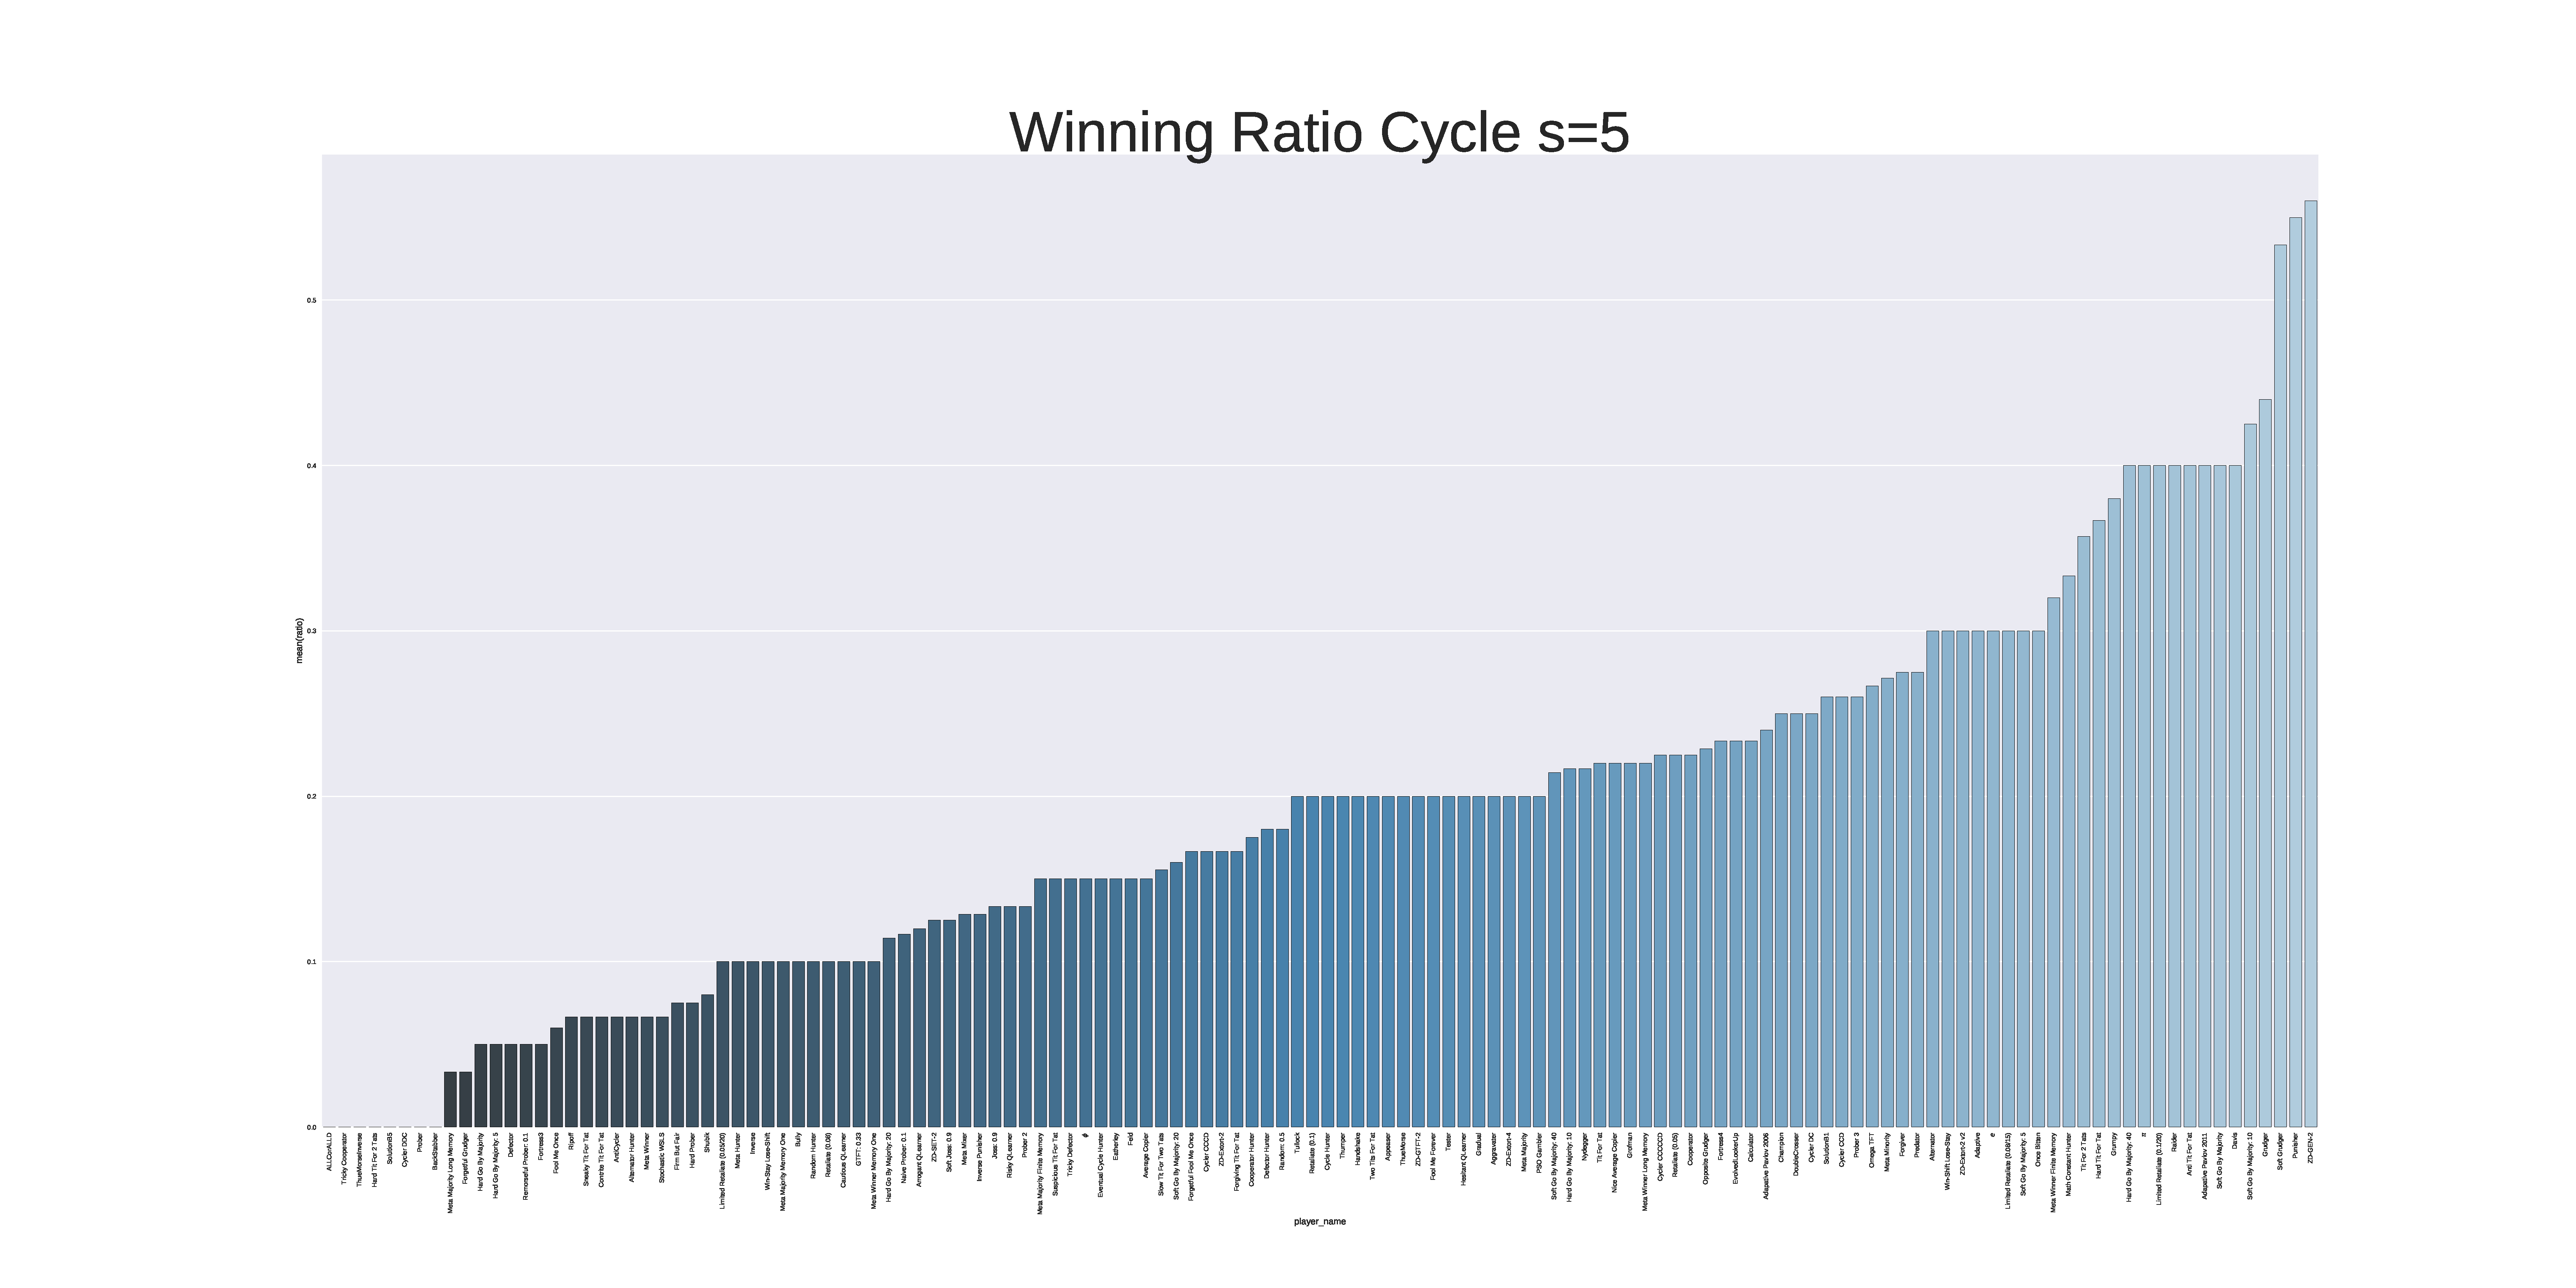
\includegraphics[width=\linewidth]{appendix/winners-cycle_five.pdf}
    \caption{Winning ration cycle s=5.}
    \end{subfigure}
\hfill
    \begin{subfigure}[t]{1\textwidth}\centering
    \centering
        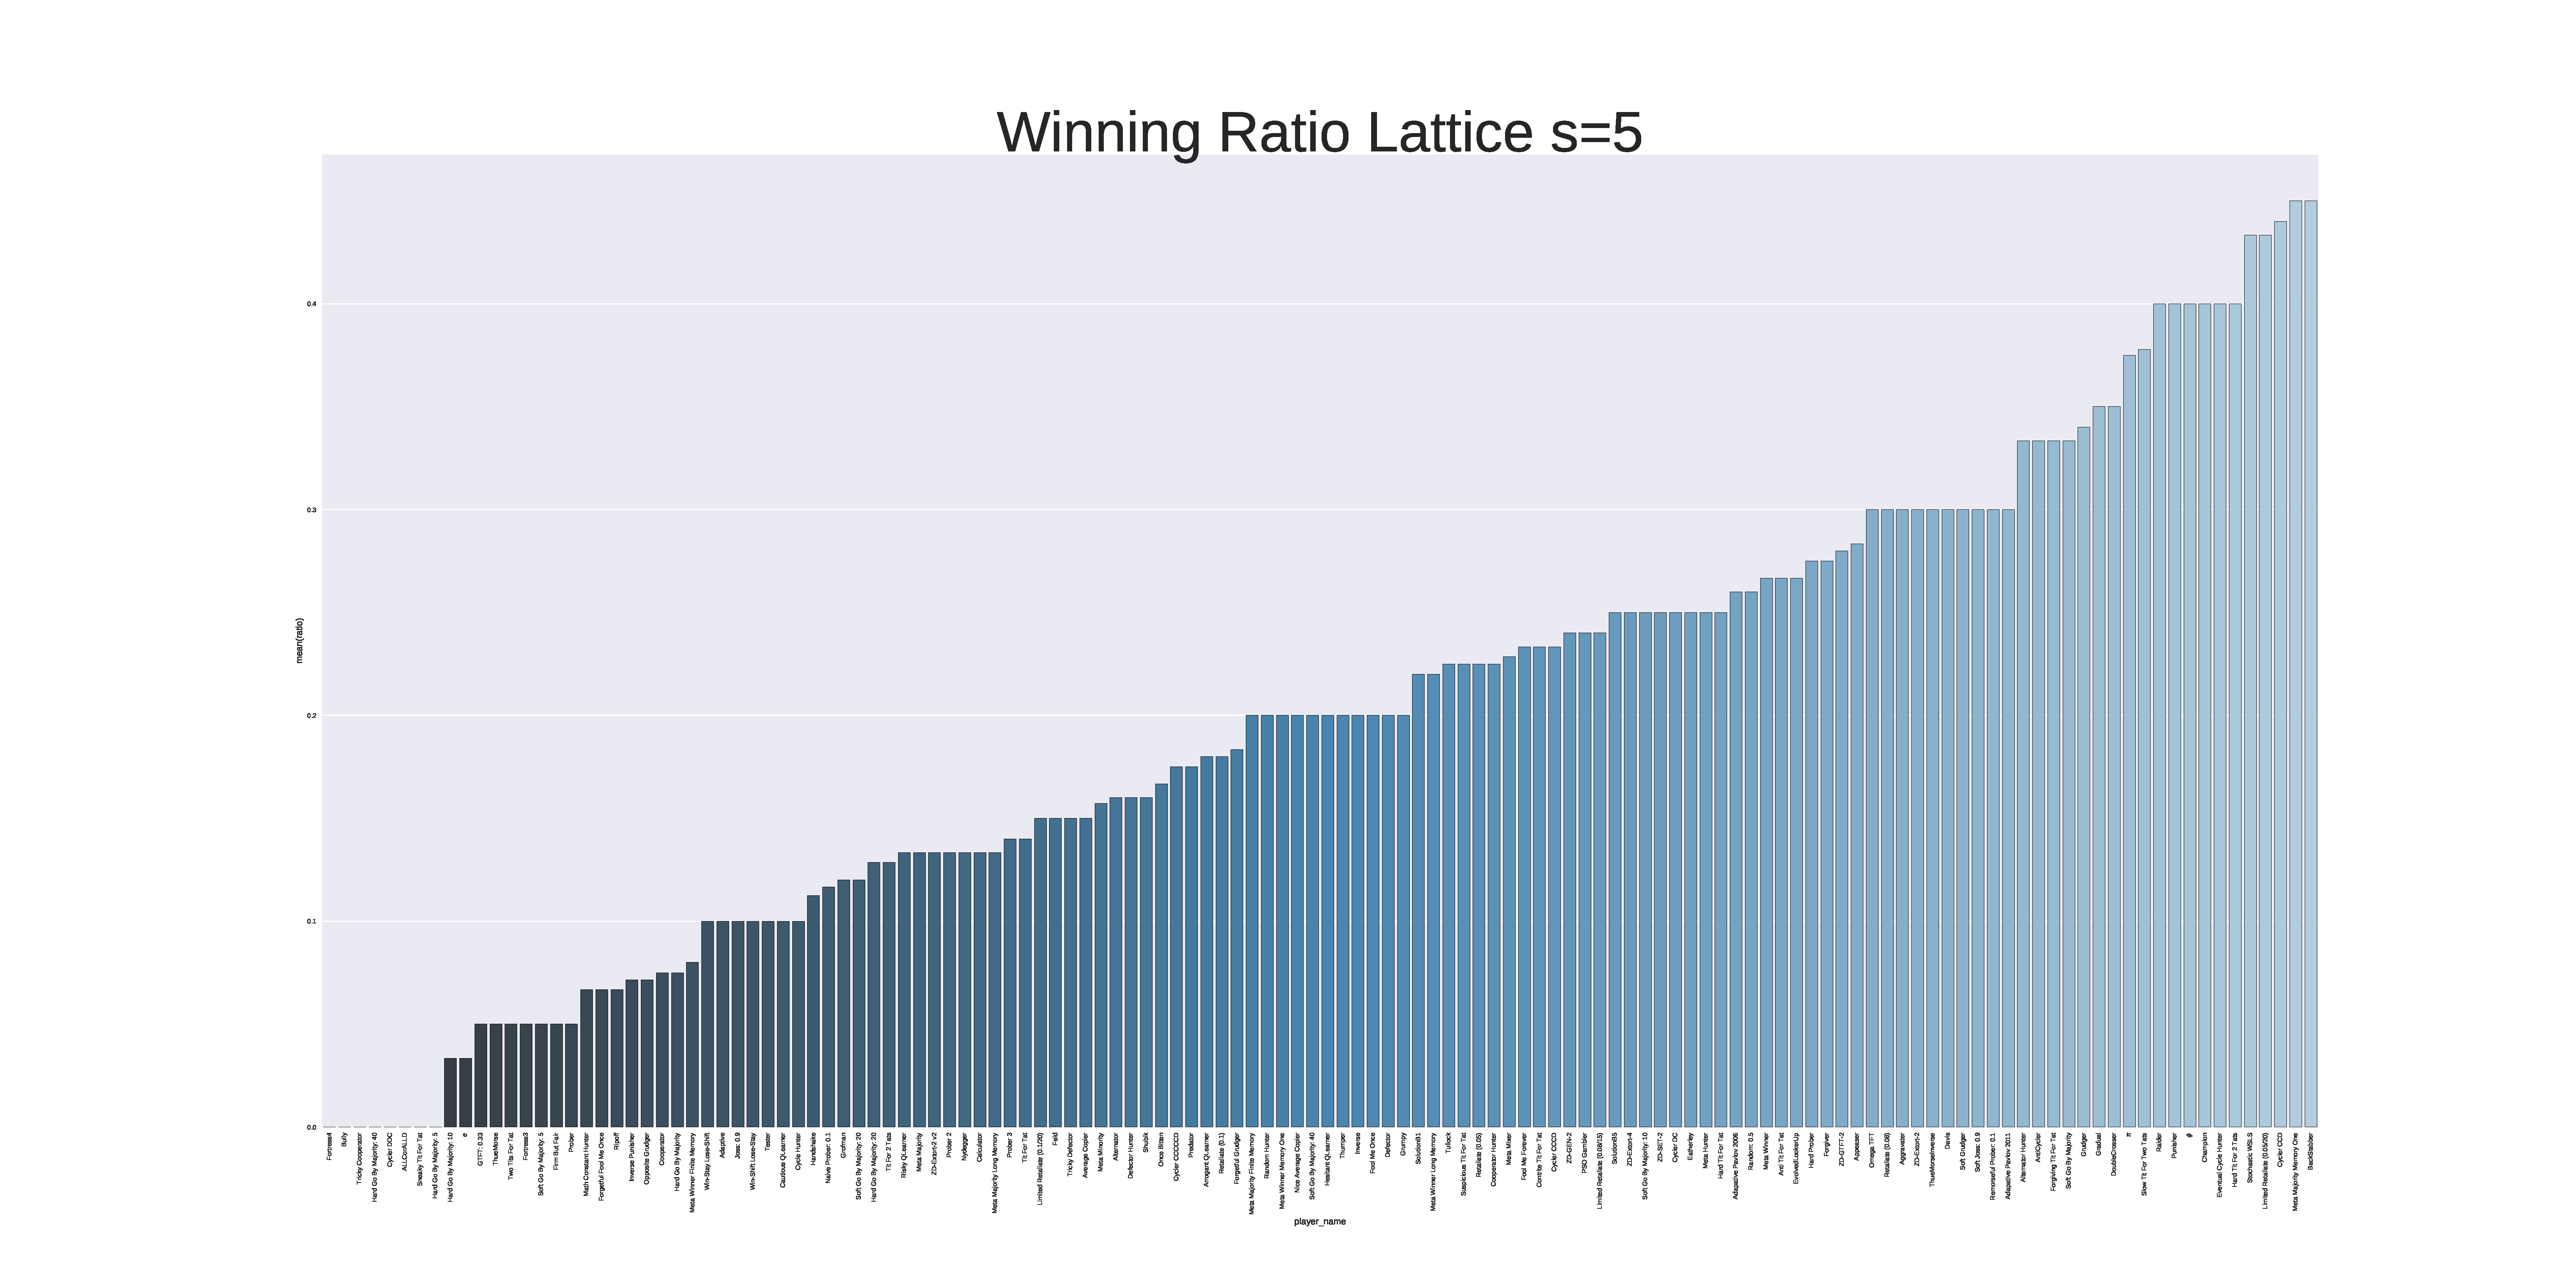
\includegraphics[width=\linewidth]{appendix/winners-lattice_five.pdf}
    \caption{Winning ration lattice s=5.}
    \end{subfigure}
\hfill
    \begin{subfigure}[t]{1\textwidth}\centering
    \centering
        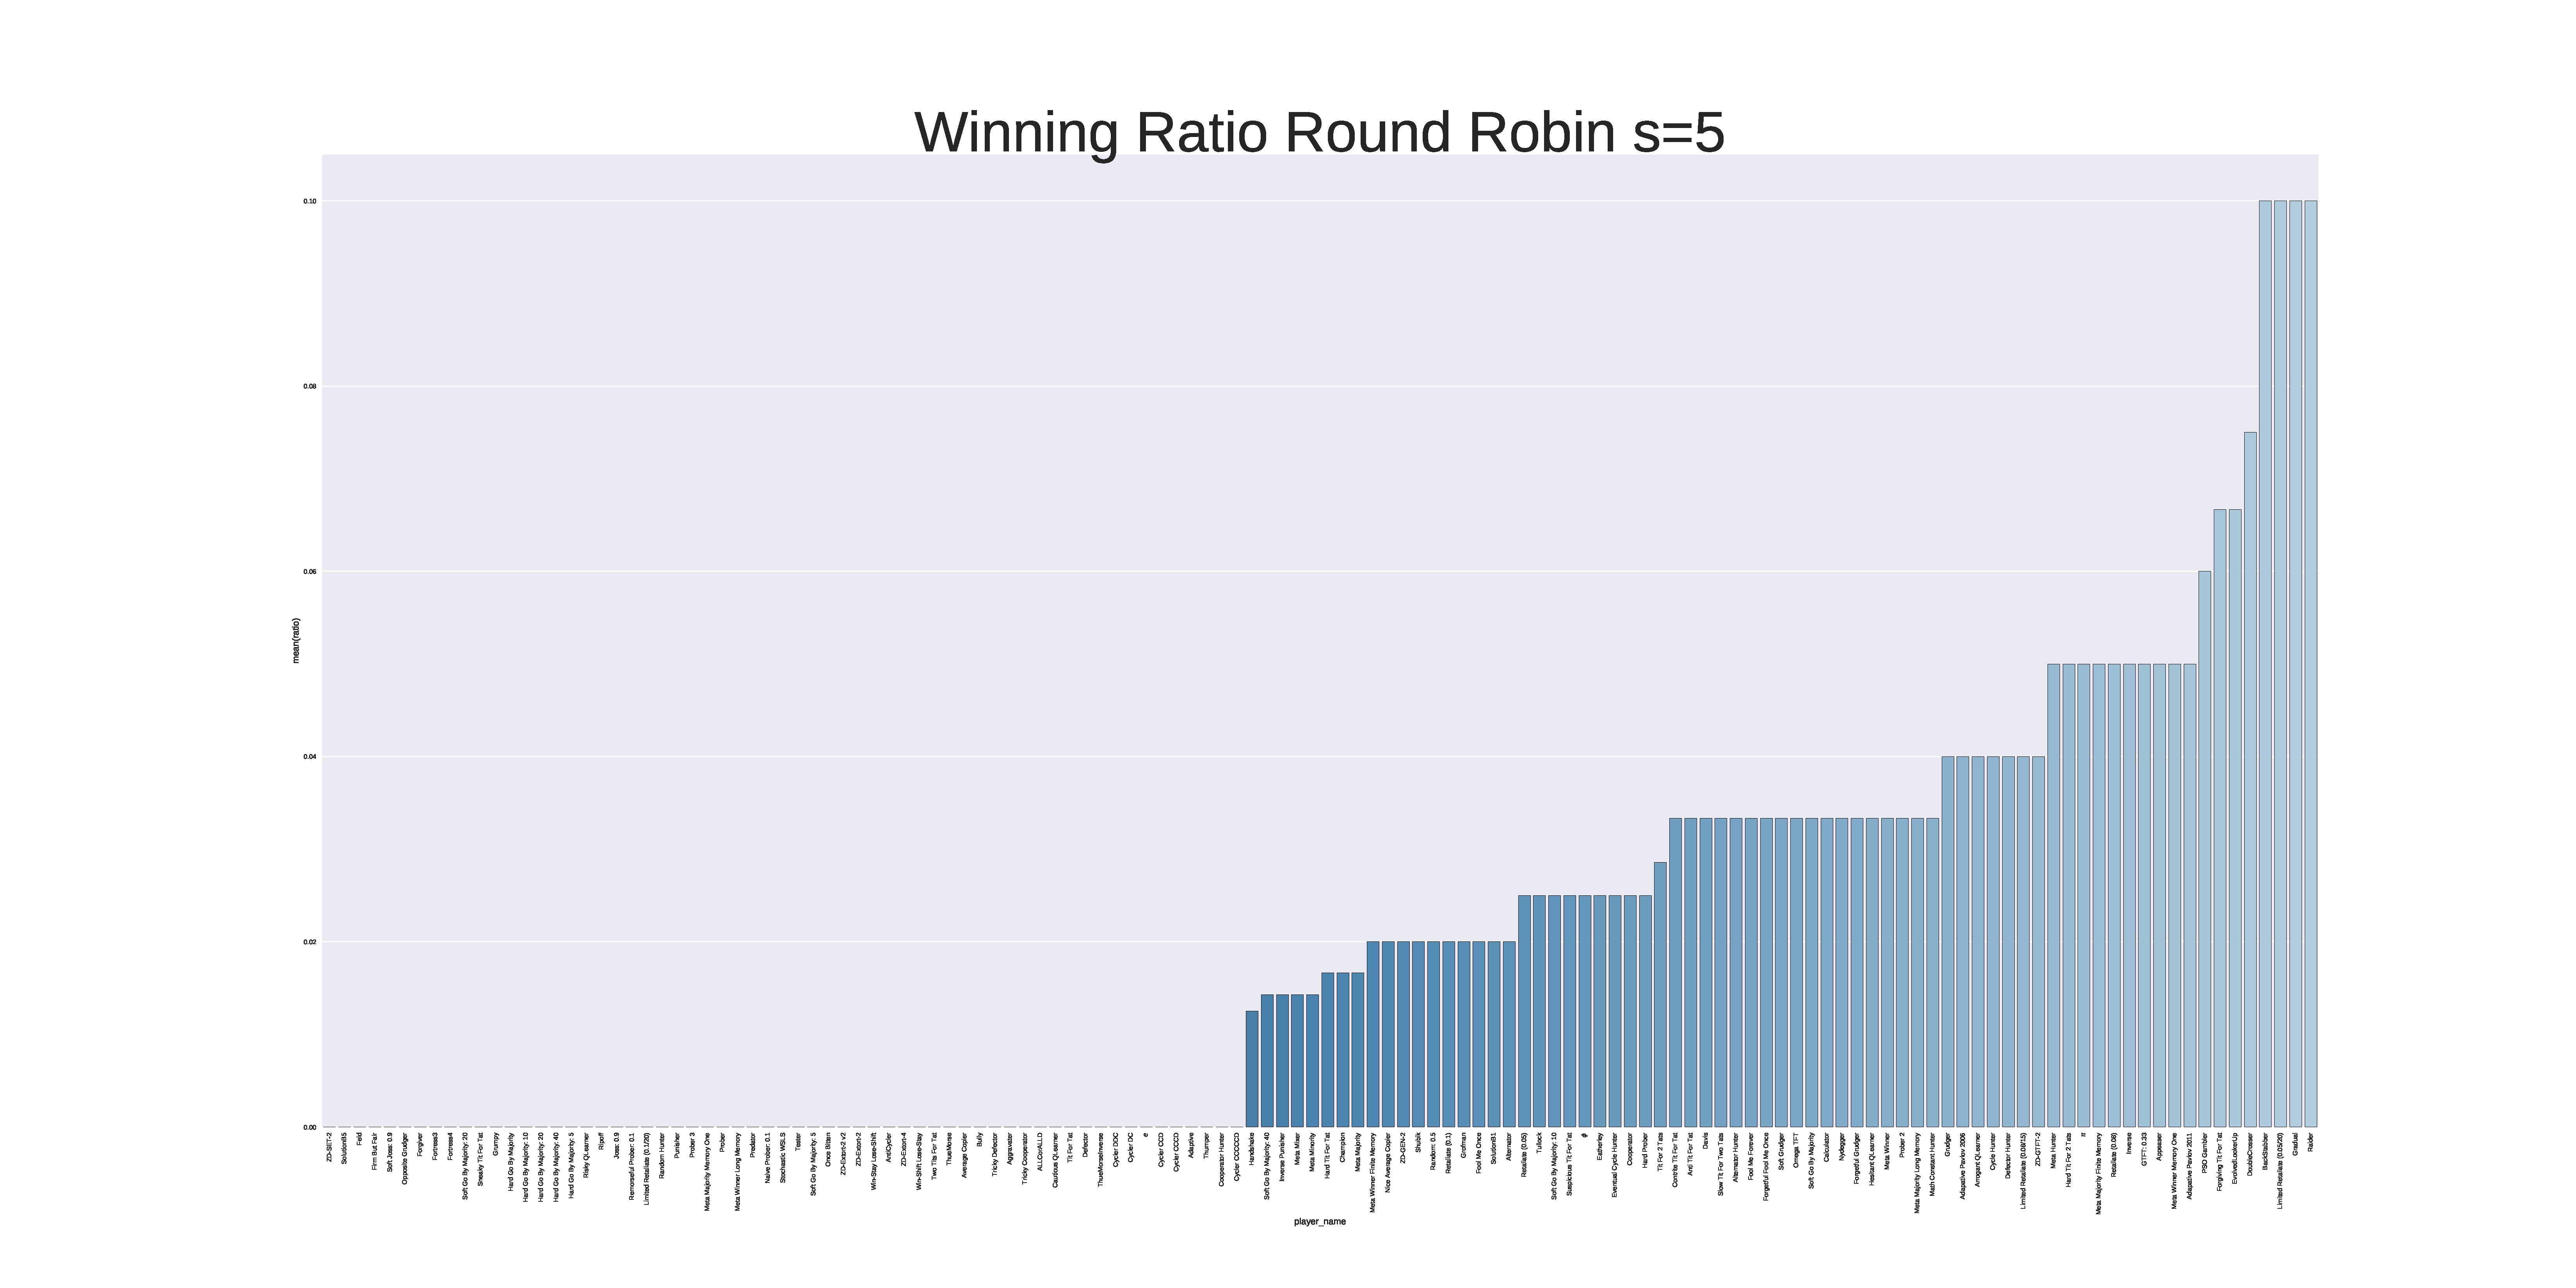
\includegraphics[width=\linewidth]{appendix/winners-rr_five.pdf}
    \caption{Winning ration round robin s=5.}
    \end{subfigure}
\caption{Winning ratio for all three topologies s=5.}
\label{fig:winning-five}
% Why are these plots bar plots? Should they just be scatter plots?
% Same comment for all of them.
\end{figure}

\begin{figure}[H]
\centering
    \begin{subfigure}[t]{1\textwidth}
    \centering
        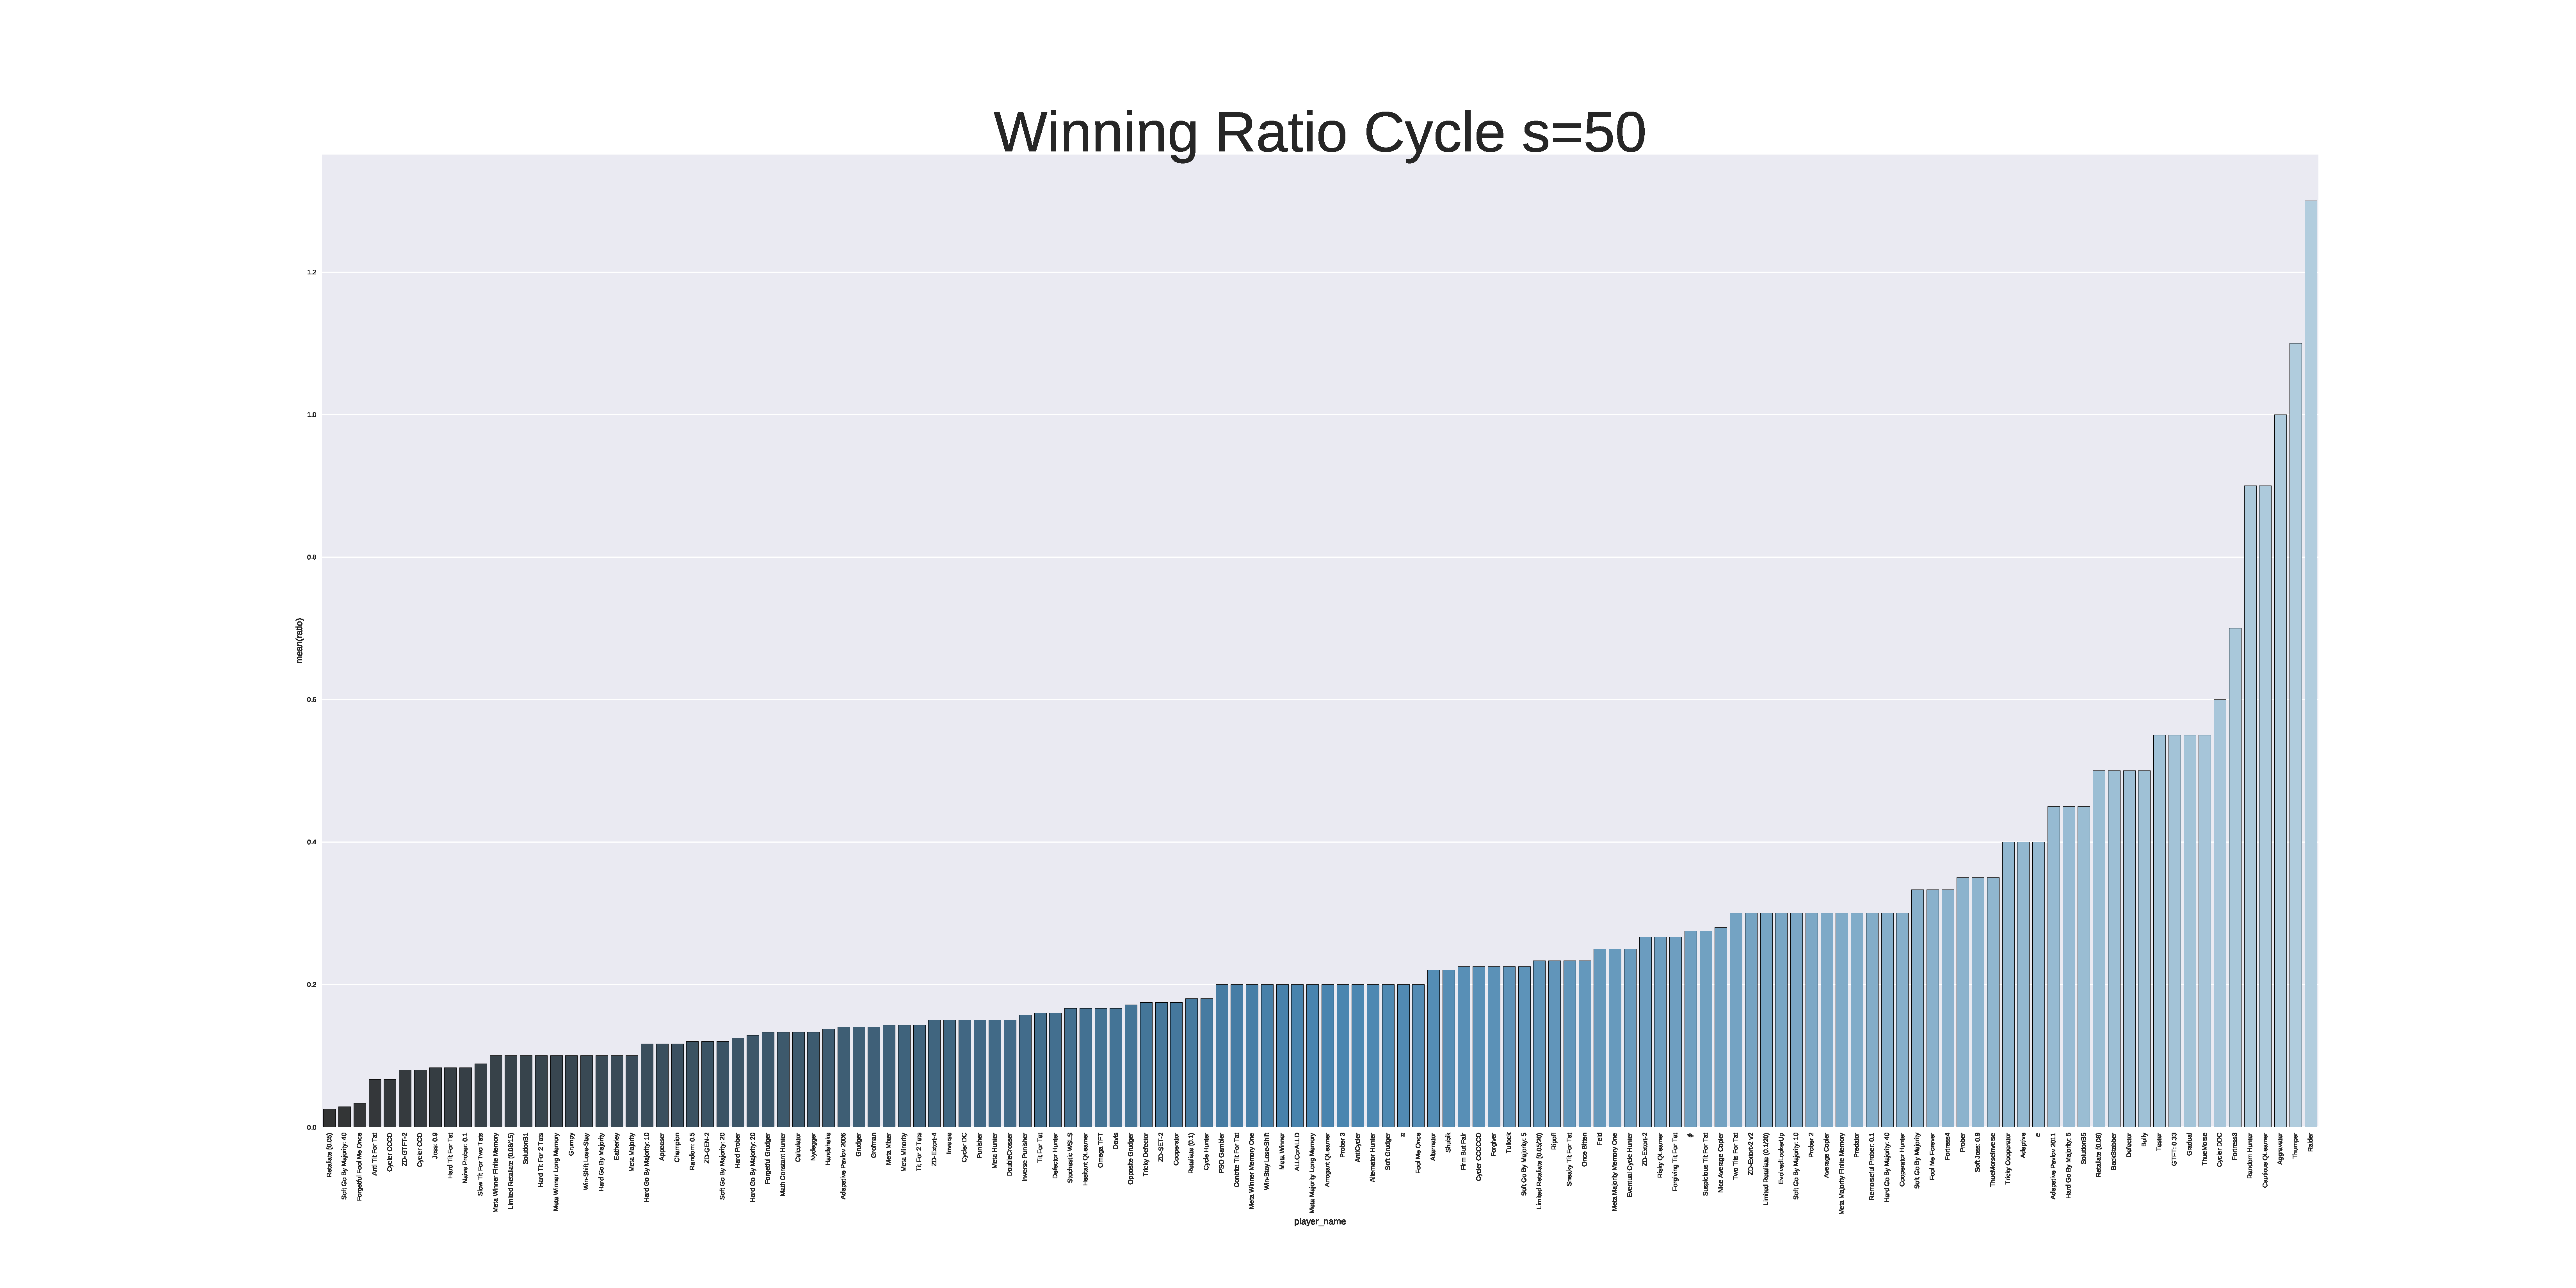
\includegraphics[width=\linewidth]{appendix/winners-cycle_fifty.pdf}
    \caption{Winning ration cyclic s=50.}
    \end{subfigure}
\hfill
    \begin{subfigure}[t]{1\textwidth}\centering
    \centering
        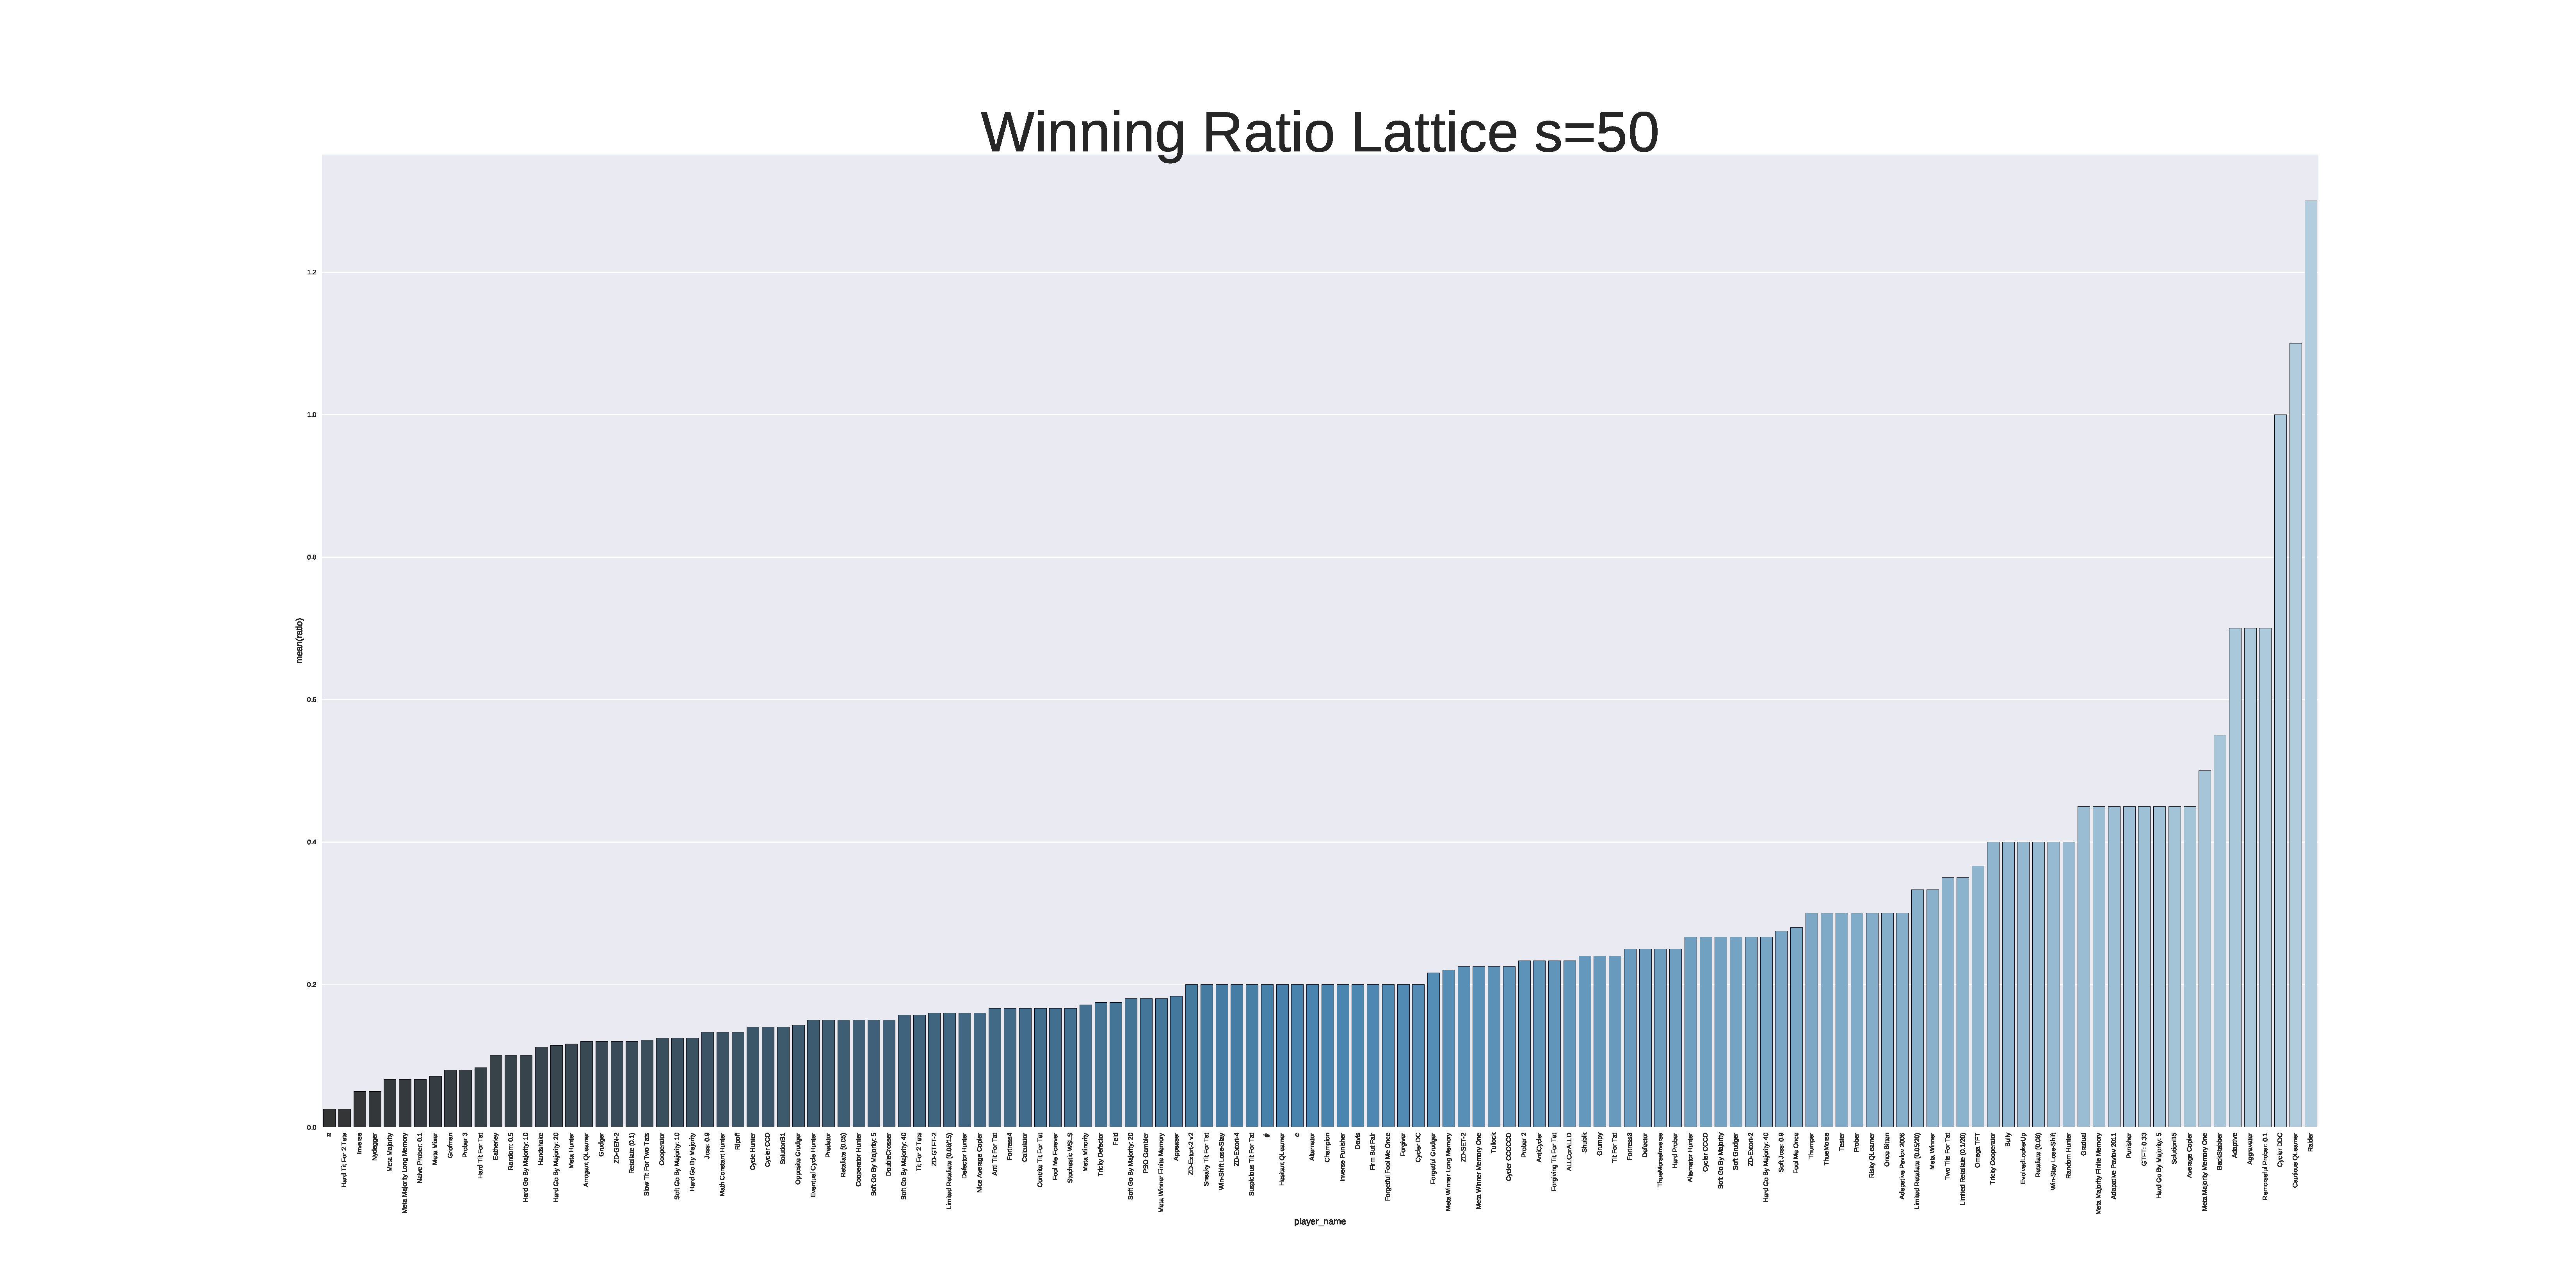
\includegraphics[width=\linewidth]{appendix/winners-lattice_fifty.pdf}
    \caption{Winning ration lattice s=50.}
    \end{subfigure}
\hfill
    \begin{subfigure}[t]{1\textwidth}\centering
    \centering
        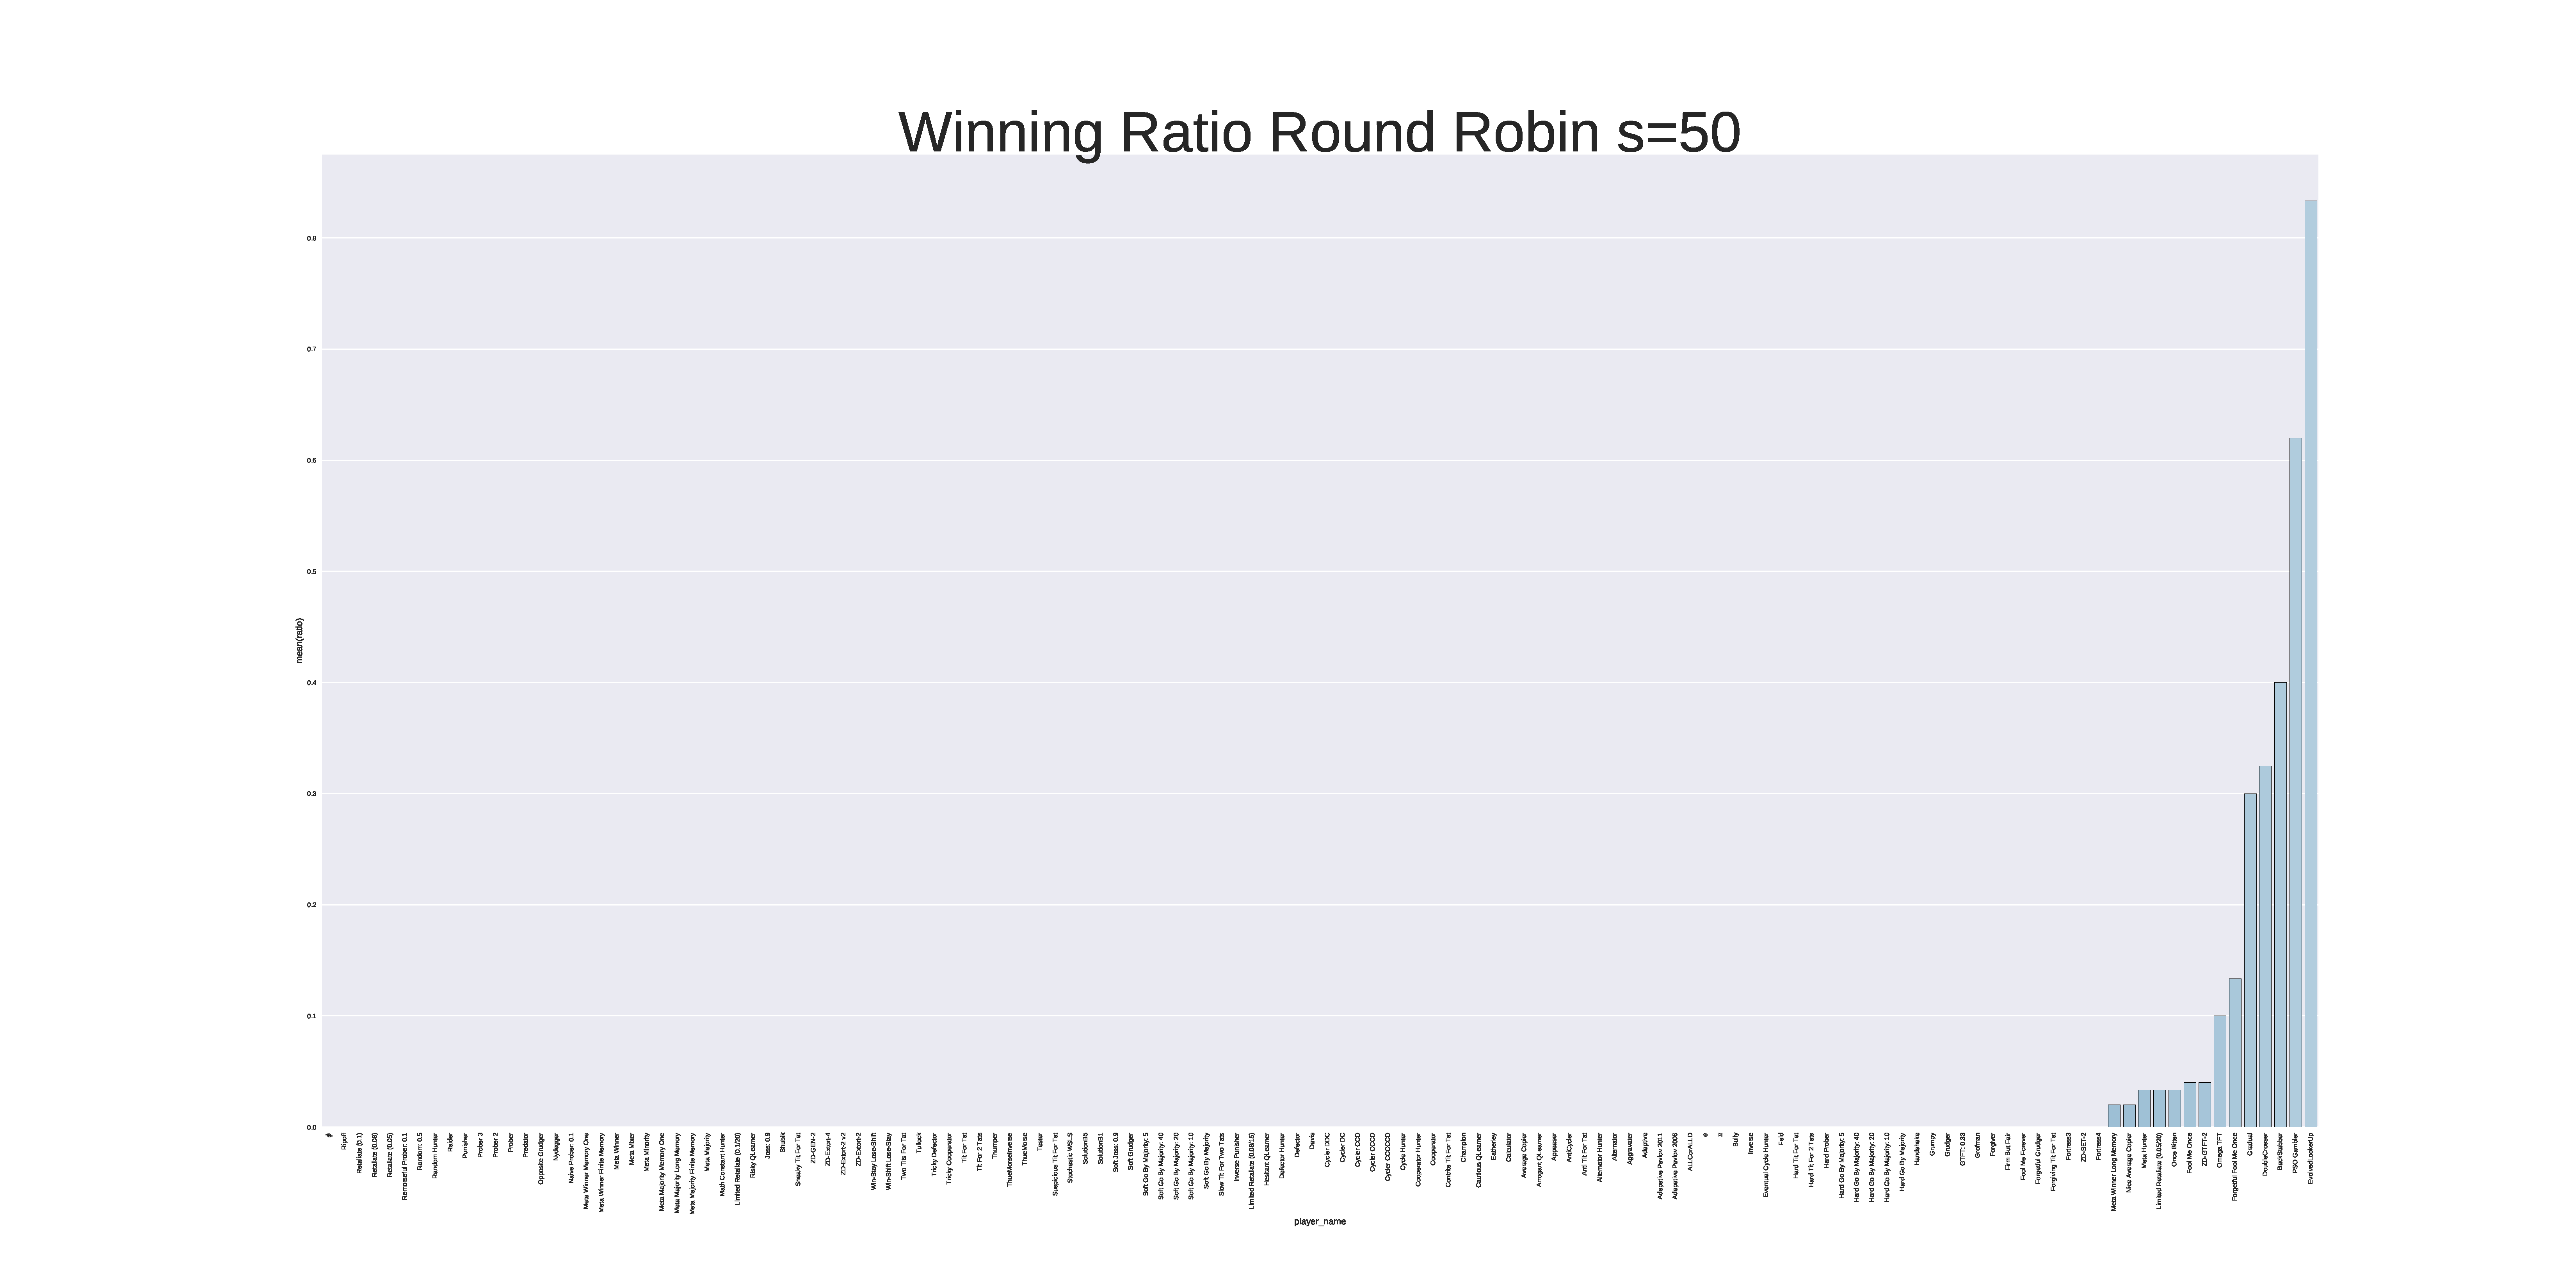
\includegraphics[width=\linewidth]{appendix/winners-rr_fifty.pdf}
    \caption{Winning ration round robin s=50.}
    \end{subfigure}
\caption{Winning ratio for all three topologies s=50.}
\label{fig:winning-fifty}
\end{figure}

\chapter{Second Appendix Title}

\lipsum[1-2]
